% Figure T3, generated by experiments/t3_llm_activations.py.
\begin{figure}[t]
  \centering
  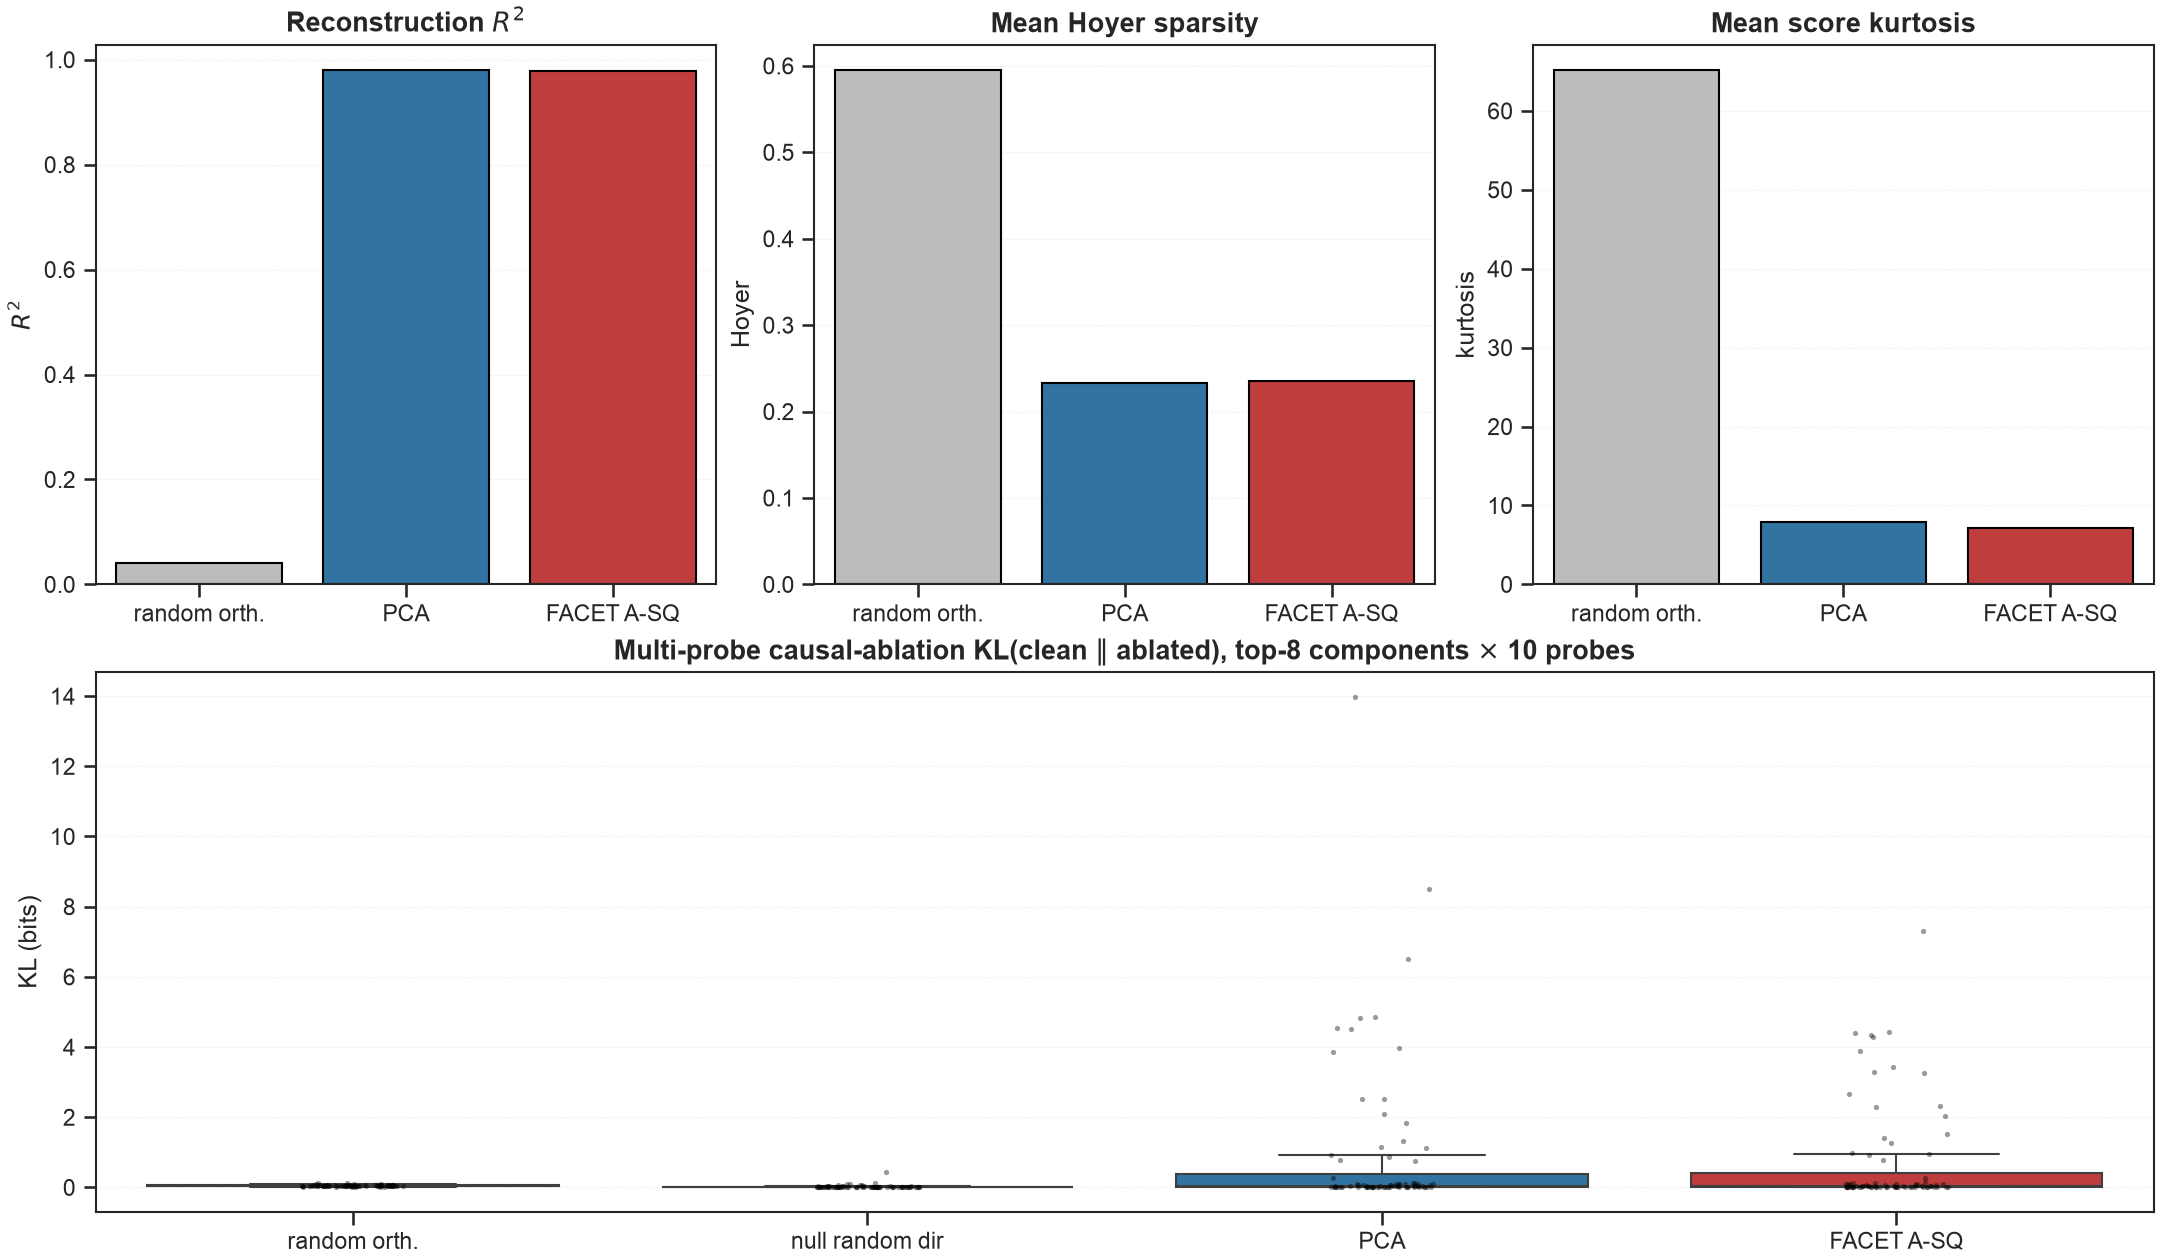
\includegraphics[width=\linewidth]{../shared/figures/generated/t3_llm_activations.png}
  \caption{\textbf{T3, GPT-2 small residual-stream activations.} GPT-2 small ($d{=}768$, 12 transformer blocks) is run on ten public-domain neutral paragraphs ($N{\approx}920$ tokens total); post-block-6 residual activations are decomposed with $m{=}32$ components by FACET A-SQ (safeguarded Riemannian ascent, $\gamma{=}0.15$), PCA (top-$m$ eigenvectors of $HH^\top$), and a random orthogonal baseline. \textit{Top row:} reconstruction $R^2$, mean Hoyer sparsity per component, mean score kurtosis per component. FACET and PCA both recover $\approx\!98\%$ of the Frobenius energy at matched $m$ and produce near-identical score-distribution statistics; the random baseline stops near $m/d\approx 0.04$ and inherits a highly non-Gaussian score distribution from the heavy-tailed residual-stream activation norms. \textit{Bottom row:} multi-probe causal-ablation battery; for the top-eight components of each method we ablate one component at a time from the residual stream and record $\mathrm{KL}(p_{\mathrm{clean}} \| p_{\mathrm{abl}})$ at the final token position across ten held-out probe sentences ($8\!\times\!10{=}80$ measurements per method). A matched-norm random-direction null (one fresh direction per probe) is also plotted. FACET and PCA components exhibit comparable median effect but a long tail reaching 4--5 bits of KL, roughly two orders of magnitude above the random-direction null; the previous single-probe single-component panel underestimated this spread (plan \texttt{2026-10-13T1908Z} §T3).}
  \label{fig:t3-llm-activations}
\end{figure}
